\chapter{再帰、非平衡秩序、イジングスピン}

\lectureoverview{部屋の半分から放出された気体は平衡へと急速に進むが、可逆的な力学によれば、十分に長い時間発展は例外的な状態への回帰もまた生じなければならない。我々は相空間体積から回帰時間を見積もり、再帰を宇宙の説明されない低エントロピーな始まりから切り離し、そこから生じる難題を用いてボルツマン脳、整合的な歴史、エネルギー流によって維持される生命について議論する。次に磁気秩序へと移る。独立な二状態スピンは厳密に解ける準備運動を与える。組み合わせ論が分配関数を決定し、磁化は双曲線正接となる。隣接相互作用がついにアップ--ダウン対称性を回復し、一次元イジング模型へと導く。}

\section{やがて戻ってくる部屋いっぱいの空気}

部屋の左半分にすべての空気がある状態から始める。この状態は仕切りによって用意できる。右半分を真空にし、空気を左側に置き、その後壁を取り除く。気体は部屋中に急速に広がり、熱平衡に近づく。エントロピーは増大する。驚くべきことは何も起こっていない。

次に部屋を密閉したまま待つ。百万回連続の表は極めて起こりにくいコイントスの記録であるが、無期限に繰り返される実験はやがて極めて起こりにくい記録を生み出す。同じ論理が気体にも当てはまる。遠いある時刻に、その分子のすべてが再び左半分に、あるいは同程度に特別な領域に見出されるであろう。そのような回帰がポアンカレ再帰である。

正確な定理はこの描像よりやや慎重である。力学が相空間体積を保存する有限測度の相空間領域に対して、ほとんどすべての初期点はその出発点にいくらでも近く戻る。\emph{すべての分子が左半分にある} といった巨視的な言明はより容易である。それは軌道が有限の粗視化された領域に再び入ることだけを問い、すべての分子座標が正確に戻ることを要求しない。実際的な問題は、それにどれだけの時間がかかるかである。

\subsection{高次元の相点}

\(N\) 個の古典粒子に対して、相空間は \(6N\) 個の座標をもち、
\begin{equation}
 \Gamma=(\bm x_1,\ldots,\bm x_N;\bm p_1,\ldots,\bm p_N).
 \label{eq:sm8-phase-point}
\end{equation}
位置は部屋によって有界である。固定された全エネルギーでは、運動量もまた有界である。なぜなら、一つの粒子が任意に大きなエネルギーを運ぶことなく任意に大きな運動量を運ぶことはできないからである。したがって、許されるエネルギー殻は再帰の議論の仮定の下で有限の測度をもつ。

相点は決定論的に運動するが、多体系の気体ではその運動はカオス的である。ビリヤード球の衝突の連続におけるように、近くの軌道は速やかに分離する。粗視化の後、長い軌道はアクセス可能な領域全体をさまようように見える。

\begin{figure}[t]
\centering
\includegraphics[width=0.90\textwidth]{lecture_08_figure_02.png}
\caption{模式的な相空間領域とその中をさまよう複雑な軌道。図は意図的に低次元であり、実際の気体は \(6N\) 次元空間に存在する。}
\lectureframe{00:06:41}
\end{figure}

低次元のスケッチは直ちに我々を誤りへと誘う。特別な状態が描かれた長方形の半分を占めるなら、気体はその時間の半分をそこで過ごすべきだと言うかもしれない。しかし \emph{すべての分子が左半分にある} という条件は、相点の一つの座標だけでなく、すべての位置座標を拘束する。

一次元空間を運動する二つの粒子だけを考え、座標を \(x_1\) と \(x_2\) とする。それらの配置空間は正方形である。\(x_1<L/2\) を要求すると正方形の半分が選ばれ、\(x_1<L/2\) と \(x_2<L/2\) の両方を要求すると四分の一が選ばれる。
\begin{equation}
 P_2=\frac{1}{2}\frac{1}{2}=\frac{1}{4}.
 \label{eq:sm8-two-particle-quarter}
\end{equation}

\begin{figure}[t]
\centering
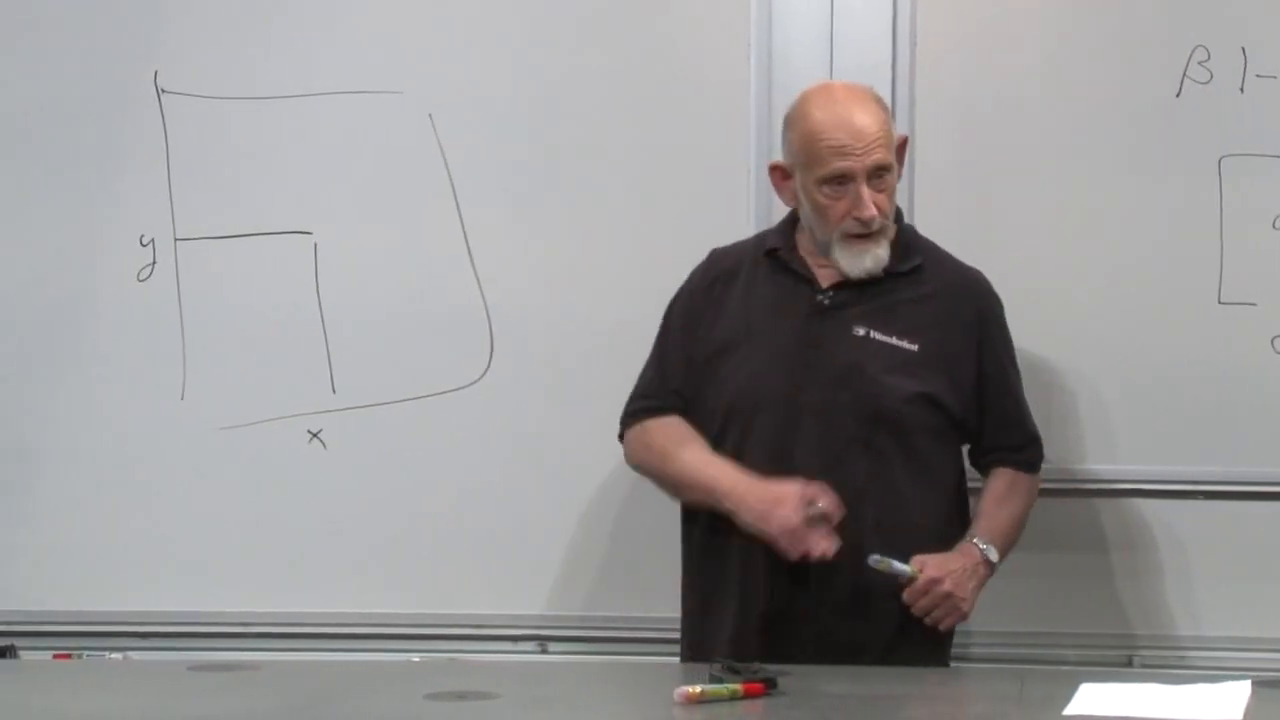
\includegraphics[width=0.90\textwidth]{lecture_08_figure_07.png}
\caption{二つの一次元粒子に対して、より小さな正方形は両方の座標が部屋の選ばれた半分にある配置を表す。}
\lectureframe{00:07:08}
\end{figure}

三つの粒子では \(1/2^3\) となり、\(N\) 個の粒子では
\begin{equation}
 P_{\mathrm{half}}(N)
 =\left(\frac{1}{2}\right)^N.
 \label{eq:sm8-half-probability}
\end{equation}
指数がすべての要点である。二分の一という因子は普通である。巨視的な粒子数で二分の一を累乗したものは、普通の直観を超えている。

\begin{classroomqa}
\audiencequestion{分子は他の空間方向ももつので、答えは \(1/3^N\) であるべきか。}
\lecturerresponse{それは課される条件に依存する。唯一の問いがすべての粒子が仕切りの左側にあるかどうかであるなら、各粒子は一つの二値条件を満たし、答えは \(2^{-N}\) である。利用可能な位置空間の別の独立な割合を拘束すれば、別の因子が与えられる。
\lecturetimestamp{00:07:47--00:08:05}}
\end{classroomqa}

\section{相体積、エントロピー、再帰のスケール}

同じ見積もりは、半分という言い方を参照せずに書くこともできる。部屋が通常の空間体積\(V\)を持ち、\(v\)を、すべての分子が見出されることを要求するより小さな領域とする。二つのマクロ状態に共通な運動量因子を無視すると、利用可能な配置空間体積は
\begin{equation}
 \Omega_{\mathrm{room}}\propto V^N,
 \qquad
 \Omega_{\mathrm{small}}\propto v^N.
 \label{eq:sm8-config-volumes}
\end{equation}
である。したがって、小さなマクロ状態に費やされる長時間の割合は
\begin{equation}
 P(v)
 =\frac{\Omega_{\mathrm{small}}}{\Omega_{\mathrm{room}}}
 =\left(\frac{v}{V}\right)^N.
 \label{eq:sm8-volume-ratio}
\end{equation}
となる。

\begin{figure}[t]
\centering
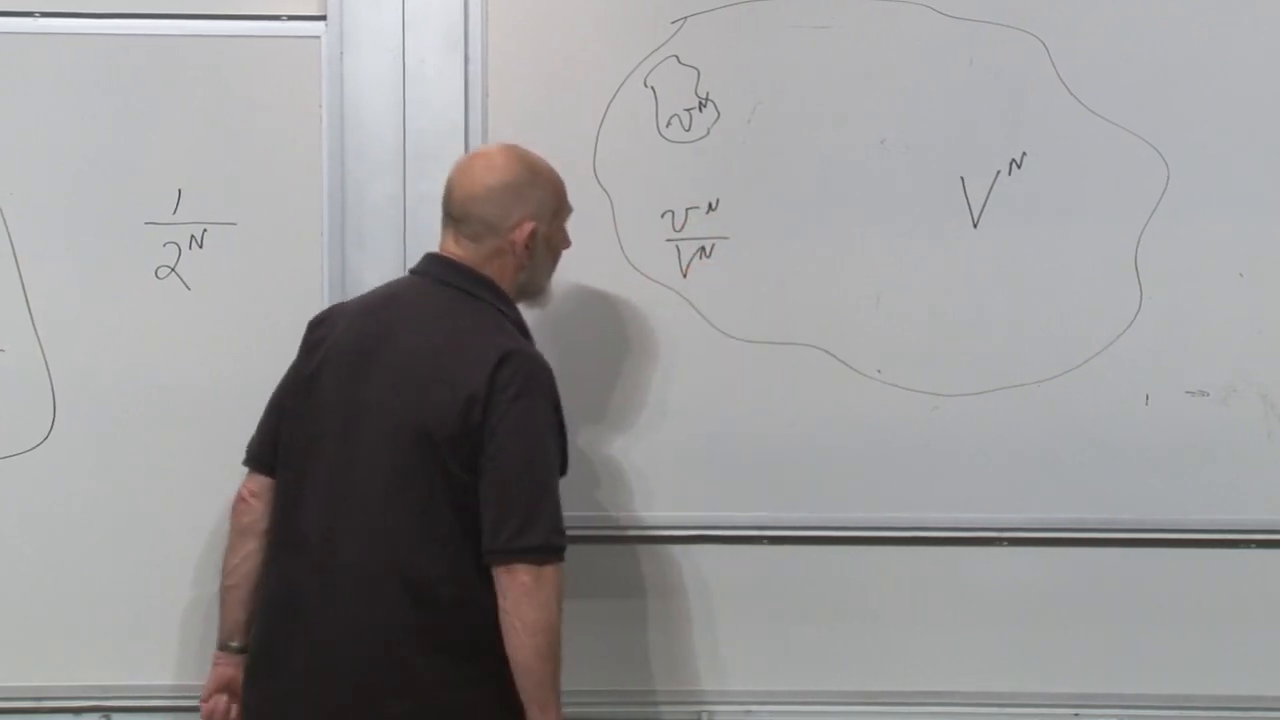
\includegraphics[width=0.90\textwidth]{lecture_08_figure_08.png}
\caption{黒板の一般的な相体積の描像：アクセス可能な領域\(V^N\)の内部にある小さな領域\(v^N\)があり、その比は\(v^N/V^N\)である。}
\lectureframe{00:10:44}
\end{figure}

\(k_B=1\)とする単位系では、エントロピーはアクセス可能な相体積の対数である。\(S_A=\log\Omega_A\)を拘束されたマクロ状態のエントロピー、\(S_{\rm eq}=\log\Omega_{\rm eq}\)を平衡状態のエントロピーとすると、
\begin{equation}
 \begin{aligned}
 P(A)
 &=\frac{\Omega_A}{\Omega_{\rm eq}}\\
 &=\exp\!\left(S_A-S_{\rm eq}\right)\\
 &=e^{-\Delta S},\\
 \Delta S&=S_{\rm eq}-S_A.
 \end{aligned}
 \label{eq:sm8-entropy-probability}
\end{equation}
である。半部屋状態では\(\Delta S=N\log 2\)であり、\eqref{eq:sm8-entropy-probability}は正確に\(2^{-N}\)に帰着する。略記\(P\sim e^{-S_{\rm eq}}\)が適切なのは、特別な領域のエントロピーを固定された基準として扱っている場合だけであり、物理的に意味のある指数はエントロピー欠損\(\Delta S\)である。

\begin{classroomqa}
\audiencequestion{これは相空間全体ではなく配置空間の体積なのか。}
\lecturerresponse{この比較に関しては、そのとおりである。位置に関する条件を課しながら、運動量分布は同じ温度のままにしているので、共通の運動量空間因子は相殺される。完全に一般的な再帰の記述は相空間を用いるが、この特定の確率は配置空間の比から計算できる。
\lecturetimestamp{00:11:21--00:11:40}}
\end{classroomqa}

系がその詳細な位置についての記憶を、微視的な相関時間または混合時間\(\tau_{\rm mix}\)で失うとしよう。そのとき、確率\(P(A)\)の稀な領域は
\begin{equation}
 \tau_{\rm rec}
 \sim \frac{\tau_{\rm mix}}{P(A)}
 \sim \tau_{\rm mix}e^{\Delta S}.
 \label{eq:sm8-recurrence-time-general}
\end{equation}
の尺度で遭遇される。半部屋条件では、
\begin{equation}
 \tau_{\rm rec}\sim\tau_{\rm mix}2^N.
 \label{eq:sm8-recurrence-time-half}
\end{equation}
である。講義では、意図的に粗い部屋サイズの見積もり\(N\sim10^{30}\)を用いており、記憶に残る尺度
\(\tau_{\rm rec}/\tau_{\rm mix}\sim2^{10^{30}}\)
が得られる。通常の大気密度では、部屋は\(10^{27}\)個の分子に近いが、\(10^{30}\)を\(10^{27}\)に置き換えても結論は何も変わらない。再帰時間は宇宙の年齢よりも想像を絶するほど大きいままである。

\begin{classroomqa}
\audiencequestion{再帰時間はどのような単位で測られるのか。秒から時間へ、あるいは極端に短い単位へ変えると、結論は変わりうるのか。}
\lecturerresponse{次元を持つ前因子は\(\tau_{\rm mix}\)であり、巨大な数は無次元の比\(\tau_{\rm rec}/\tau_{\rm mix}\)である。秒を時間に変えることは通常の換算因子で割ることであり、それは\(2^{10^{30}}\)に比べて無視できる。隅への個々の訪問の継続時間は分子速度に依存する。この見積もりが関わるのは、その訪問がどれほど稀に始まるかである。量子再帰定理も存在するが、ここでは必要ない。
\lecturetimestamp{00:17:24--00:19:18}}
\end{classroomqa}

\begin{classroomqa}
\audiencequestion{どの実験も待つことなど到底できない時間を計算する目的は何か。}
\lecturerresponse{要点は概念的である。それは、閉じた力学系がどのような意味で可逆性を保つかを教えてくれる。系はほとんどすべての時間を平衡状態の近くで過ごすが、十分に長い尺度では、より低いエントロピーへ向かう揺らぎも起こす。したがって第二法則は、特別な初期データについての圧倒的に確からしい主張であり、逆向きの運動を禁じる微視的方程式ではない。
\lecturetimestamp{00:15:12--00:16:35}}
\end{classroomqa}

\section{可逆性と特別な始まり}

意図的に、小さな半部屋領域から始める。隣接するほとんどすべての軌道は直ちにそこを離れる。なぜなら、内部よりも外部のはるかに多くの相体積が存在するからである。気体は速やかに広がり、その後、戻るまでに途方もない時間を待つ。速やかな緩和と長い待ち時間の間のこの非対称性は、可逆的な力学に反しない。

速やかな脱出の時間反転は、待ち時間全体ではない。それは、平衡状態に見える分子速度がたまたま整い、気体が部屋の半分へ\emph{swooshes}と流れ込む、短く、驚異的にうまく調整されたエピソードである。通常の脱出の終わりにすべての運動量を反転させれば、気体は脱出を逆向きにたどる。長い待ち時間とは、その特別な入射速度パターンが自発的に生じるのに必要な時間である。

\begin{classroomqa}
\audiencequestion{時間対称性とは、隅への遅い再帰が、そこからの元の脱出と同じだけ長くかかることを意味するのか。}
\lecturerresponse{いいえ。脱出をその正確な時間反転と比較せよ。どちらも速やかである。膨大な時間がかかるのは、逆向きの流れ込みを開始させる正確な入射揺らぎを、平衡状態で待つことである。途方もなく長い記録の上では、平衡から離れる逸脱は、対称な局所履歴をもって両方の時間方向に起こる。
\lecturetimestamp{00:20:46--00:21:58}}
\end{classroomqa}

したがって、再帰の議論は時間の矢の一部しか説明しない。系が低エントロピーの領域から始まった\emph{という条件のもとで}、エントロピーが通常は増大する理由を説明する。しかし、初期条件がなぜ特別であったかは説明しない。宇宙論では、この欠けた前提が中心的な問いとなる。なぜ観測可能な宇宙は、その重力相空間のこれほど例外的に小さな領域から始まったのか。

\begin{classroomqa}
\audiencequestion{再帰は宇宙論に当てはまるか。宇宙が広がった後、十分長く待てば再帰するのだろうか。}
\lecturerresponse{その問いは避けられないが、その答えは大域的な宇宙論に依存する。有限の平衡状態空間をもつ真に閉じた系は再帰を促す。膨張する時空、重力、地平線、そして無限または非定常な状態空間は前提を変えうる。ここでの重要な教訓はより限定的である。平衡の再帰という描像それ自体は、我々が見る構造化された宇宙に対する満足な統計的説明ではない。
\lecturetimestamp{00:19:59--00:20:45}}
\end{classroomqa}

\begin{classroomqa}
\audiencequestion{再帰は、最初に気体を小さな領域に用意することに依存するのか。部屋が平衡から始まっても、空気は最終的にやはり一つの隅に集まるのか。}
\lecturerresponse{はい。再帰は閉じた系の長時間の力学に関するものであるから、平衡に見える初期状態もまれな低エントロピー揺らぎを経る。半部屋状態を用意することが重要であるのは別の理由による。それにより、既知の特別な始まりを条件として、その直後にエントロピーがなぜ増大するのかを問うことができる。
\lecturetimestamp{00:22:04--00:22:20}}
\end{classroomqa}

\section{なぜランダムな揺らぎは少なすぎることを予測するのか}

再帰を宇宙論に変えようとする試みもありうる。おそらく宇宙は永遠のほとんどを平衡で過ごし、我々の現在の世界はまれな一つの揺らぎなのだろう。この提案は鋭い統計的検証に失敗する。観測者が存在することを条件として、その観測者が他に何を見ることを期待すべきかを問うのである。

一つの惑星を作るのに十分大きな揺らぎは、極めてまれである。二つの惑星を作る揺らぎは、より大きなエントロピー不足を必要とし、さらにまれである。恒星、銀河、宇宙マイクロ波背景放射、そして長い過去について互いに整合する記録を作る揺らぎは、莫大な追加の指数分だけさらにまれである。したがって、平衡揺らぎ理論は、観測に十分な最小の揺らぎを予測するのであって、実際に観測される豊かに整合した世界を予測するのではない。その最も極端な形では、最小の観測者はボルツマン脳と呼ばれる。

論理は条件付き確率である。\(A\)を観測者サイズの揺らぎが一つ起こる事象、\(B\)を独立な第二の構造とする。両者が微小な確率\(p\)をもつならば、
\begin{equation}
 P(B\mid A)=p,
 \qquad
 P(A\cap B)=p^2.
 \label{eq:sm8-conditional-fluctuations}
\end{equation}
第一の揺らぎが起こったことを知っても、第二の揺らぎが起こりやすくなるわけではない。宝くじの類推はこの水準では正確である。以前の当選者は、次の独立な抽選で当たる確率が高くなるわけではない。したがって、観測者は自分が存在することを条件としてよいが、独立に構造化された環境を見いだしたならば、それでも驚くべきである。

\begin{classroomqa}
\audiencequestion{一つの惑星または一人のボルツマン観測者がすでに存在するとして、もう一つが存在する確率は本当に小さいのか。}
\lecturerresponse{第二の独立なまれな揺らぎに対する条件付き確率は、同じ微小な一事象確率であり、その二乗ではない。両方に対する同時確率が二乗である。まさにこの理由により、第一の観測者は自分の外側には依然として熱的無秩序を期待すべきである。配偶者、別の惑星、そして秩序だった空を見いだすことは、その観測者が孤立した平衡揺らぎとして組み立てられたという前提に反する証拠である。
\lecturetimestamp{00:26:12--00:30:27}}
\end{classroomqa}

\subsection{過去についての整合する記録}

同じ議論は歴史にも当てはまる。一致する二冊の教科書、一つの膨張史に適合する天文記録、地質層、記憶、実験ノートはすべて互いを制約する。一冊のランダムな教科書はどんな物語でも含みうる。同じ過去について一致する記録の網全体は、はるかに小さな相空間領域を占める。

教室の例では、ジョージ・ワシントンが桜の木を切り倒したというよく知られた話を用いる。その話が真実かどうかは無関係である。要点は、現在の瞬間に揺らぎから存在するに至った世界では、ある本の一文が別の記録の一致に対する力学的な理由を与えないということである。整合する相関は、単なる一瞬の偶然の証拠ではなく、共有された歴史の証拠である。

\begin{classroomqa}
\audiencequestion{ここでいう\emph{歴史的一貫性}とは何を意味するのか。}
\lecturerresponse{それは、現在の多くの記録が共通の過去の帰結として互いに整合していることを意味する。揺らぎが記録や記憶を捏造することはあり得るが、相互に整合するネットワークを捏造するには、最小限の観測者を一つ捏造するよりもはるかに大きな揺らぎが必要である。したがって再帰理論は、観測者に似た揺らぎの大多数は、我々が実際に見出している一貫性を欠くと予測する。
\lecturetimestamp{00:30:30--00:31:12}}
\end{classroomqa}

\begin{classroomqa}
\audiencequestion{宇宙は依然として閉じた系であり、その平衡化時間と再帰時間が単に極めて長いだけだということはあり得ないのか。}
\lecturerresponse{その可能性は統計的な問題を取り除かない。無限に長い歴史の上では、観測者に似た揺らぎが多数存在し、その圧倒的多数は一貫した周囲の歴史を伴わない最小限のものであろう。その集団から選ばれた観測者は、我々の観測を期待すべきではない。したがって宇宙論研究者は、ボルツマン脳問題を、再帰がすでに観測されたという主張としてではなく、宇宙論的測度と晩期モデルの検証として真剣に受け止めている。
\lecturetimestamp{00:31:13--00:32:42}}
\end{classroomqa}

\section{流れによって維持される構造としての生命}

生命は逆の困難を提起しているように見える。生物は複雑な組織を長期間維持するのであり、短命的な偶発的揺らぎのようには見えない。その解決は、第二法則が完全な閉じた系に適用されるということである。部分系は、その環境においてより大きなエントロピー増大が起こるならば、そのエントロピーを低下させ、あるいは維持してもよい：
\begin{equation}
 \dot S_{\rm total}
 =\dot S_{\rm subsystem}+\dot S_{\rm environment}\geq 0.
 \label{eq:sm8-open-system-second-law}
\end{equation}

地球は熱平衡にはない。人間の時間尺度ではほぼ定常であるが、定常は静的を意味しない。エネルギーが地球を通って流れる。太陽光が到来し、多くの過程を通じて劣化し、より低い実効温度で放射されて去る。その通過流量は、全エントロピーが増大しつつ局所的な組織を維持し得る。

管を通って流れる水は、直接的な力学的イメージを与える。その流れは持続的な渦や渦巻きを含み得る。それらは組織化された構造であるが、水流によって維持されている。両端を密閉し、流れを止めれば、水が鈍い平衡に近づくにつれて粘性が渦を消し去る。流出する水は流入する水より温かいので、より大きな系がエントロピーの勘定を支払ったことになる。

\begin{classroomqa}
\audiencequestion{生命はエントロピーを減少させるのか、そしてなぜその組織は通常の揺らぎのように現れては消えるのではなく持続し得るのか。}
\lecturerresponse{生命は局所的にエントロピーを維持し、あるいは低下させ得るが、それはさらに多くのエントロピーを外部へ排出することによってのみである。その持続は定常的な非平衡の流れ、主に地球を通る太陽エネルギーの流れに由来する。もし地球が入射および出射放射に対して密閉されていれば、やがて熱平衡に近づき、組織化された活動は停止するであろう。生命は平衡の揺らぎというよりも、流れの中の渦に近い。
\lecturetimestamp{00:32:43--00:35:42}}
\end{classroomqa}

これで我々は\emph{興味深いもの}を離れ、講義の意図的に乾いた表現を借りれば、何か退屈なもの、すなわち磁石に戻る。

\section{磁石の冷却：磁区と選ばれた方向}

統計力学は、文字通りの鉄片でない場合でも、数学的模型をしばしば磁石と呼ぶ。有用な共通の特徴は、秩序化し得る局所的自由度の集まりである。実際の磁性材料では、これらの自由度は原子磁気モーメント、電子スピン、軌道電流、または結晶単位の有効モーメントに由来し得る。

高温では熱的無秩序により局所モーメントが多くの方向を向き、正味の磁化はほとんど、あるいは全く生じない。隣接するモーメントが整列したときに低いエネルギーを持つならば、冷却によって小さな整列磁区が形成され得る。さらに冷却するとエネルギーの利得がより重要になり、相関した磁区が成長する。強磁性転移を支える系では、相関長は有限の臨界温度で巨視的になる。すると秩序相は、ゼロ磁場のエネルギーが前もって一つの方向を好まなかったにもかかわらず、一つの配向を選ぶ。

\begin{classroomqa}
\audiencequestion{N極がS極を引き付けるのだから、微視的な磁石は反平行に整列することを好むべきではないのか。}
\lecturerresponse{有効相互作用は物質に依存する。通常の双極子の直観は微視的問題のすべてではない；交換相互作用、結晶構造、競合する相互作用が重要である。強磁性材料とは、有効な低エネルギー傾向が平行秩序を好むものであり、他の材料は反平行整列を好み得る。
\lecturetimestamp{00:39:56--00:40:30}}
\end{classroomqa}

\begin{classroomqa}
\audiencequestion{モーメントが揃うためには、物質が冷却する間に外部磁場が存在しなければならないのだろうか。}
\lecturerresponse{いいえ。相互作用は磁場なしでも秩序を生み出しうる。完全に対称な理想化では、異なる方向はエネルギー的に等価であるため、実現される方向は初期揺らぎ、境界、あるいは任意に小さな迷走磁場によって選ばれる。それらの等価な方向の一つを選ぶことが自発的対称性の破れであり、巨視的秩序の出現が磁気相転移である。
\lecturetimestamp{00:40:31--00:42:33}}
\end{classroomqa}

実在の物質は複雑であるから、ここでは徹底的に単純化する。各局所モーメントは上向きか下向きのいずれかしか向けない：
\begin{equation}
 \sigma_i=+1\quad\hbox{or}\quad\sigma_i=-1.
 \label{eq:sm8-ising-spin}
\end{equation}
この模型には東も西もない。許される二つの配向は、表と裏が硬貨の二つの結果であるのと同様に、模型の定義である。その価値は微視的実在性にあるのではなく、数学的明瞭さと、多くの系に共通する秩序化現象を表現できることにある。

\begin{classroomqa}
\audiencequestion{これら二状態の対象は物理的には何なのか。それらを粒子として想像すべきなのだろうか。}
\lecturerresponse{結晶の格子点にある原子を思い描き、それぞれがスピンや微視的電流によって生じた有効磁気モーメントを持つと考えることができる。しかし模型にとっては、二値変数だけが重要である。上向きと下向きへの制限は、統計力学を簡単にするために課されている。
\lecturetimestamp{00:44:22--00:45:01}}
\end{classroomqa}

\section{外部磁場中の独立スピン}

最初の模型は互いに相互作用しない\(N\)個のスピンを含む。外部磁場\(H\)が唯一のエネルギー尺度を与え、\(\mu\)は一つのスピンのそれへの結合の強さを測る。計算で用いた符号の規約を保つ：
\begin{equation}
 \epsilon_i=\mu H\sigma_i.
 \label{eq:sm8-single-spin-energy}
\end{equation}
\(H>0\)に対して、上向きスピン\(\sigma_i=+1\)はエネルギー\(+\mu H\)を持ち、下向きスピン\(\sigma_i=-1\)はエネルギー\(-\mu H\)を持つ。したがってこの規約では、正の磁場は下向きスピンを好む。これは別の一般的な命名規約とは逆であるが、符号を一貫して用いる限り、名前には物理が依存しない。

\(n\)を上向きスピンの数、\(m\)を下向きスピンの数とする。このとき
\begin{equation}
 n+m=N,
 \qquad
 E=(n-m)\mu H.
 \label{eq:sm8-counting-energy}
\end{equation}

\begin{figure}[t]
\centering
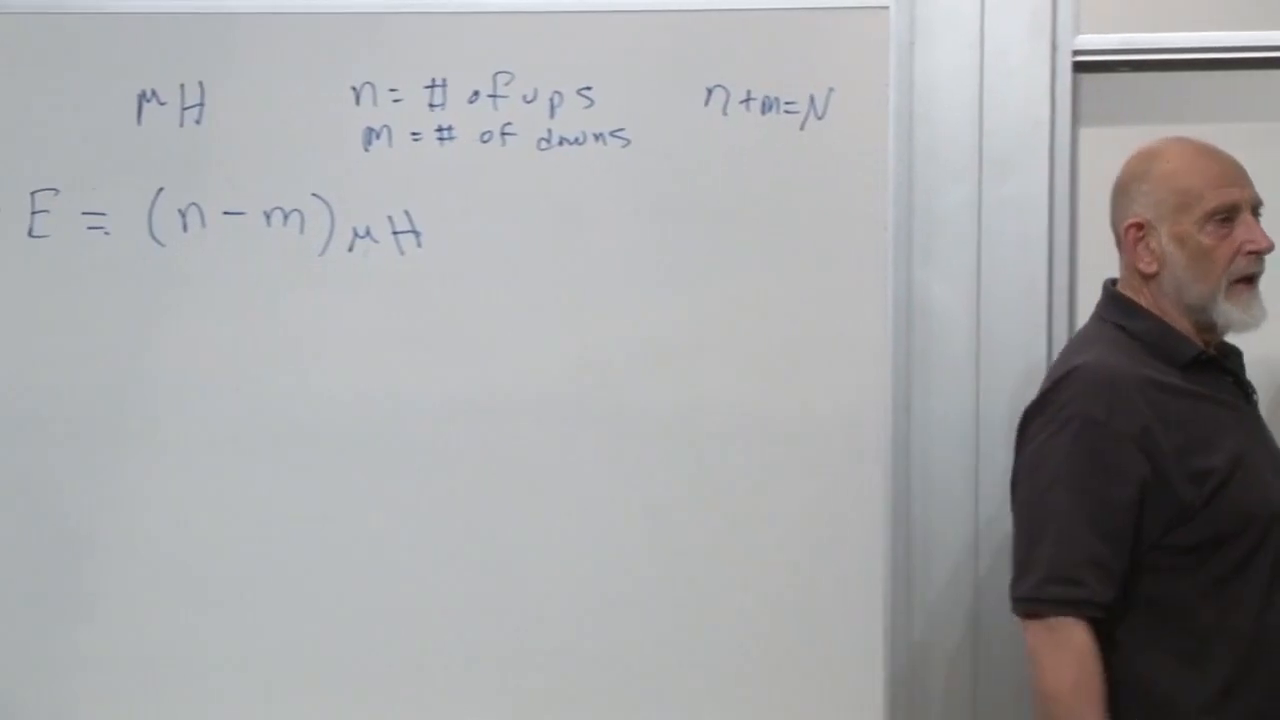
\includegraphics[width=0.90\textwidth]{lecture_08_figure_03.png}
\caption{独立スピンの設定：上向きスピン\(n\)個、下向きスピン\(m\)個、\(n+m=N\)、および\(E=(n-m)\mu H\)。}
\lectureframe{00:49:50}
\end{figure}

\begin{classroomqa}
\audiencequestion{\(H\)、\(\mu\)、\(E\)の次元は何か。\(H\)は数なのか磁場なのか。}
\lecturerresponse{\(H\)は外部から課された磁場の強さを表し、\(\mu\)は磁気モーメントを表す。それらの積\(\mu H\)はエネルギーの次元を持つ。抽象模型では、しばしばそれらを単一のエネルギー値のパラメータにまとめ、慣例的に小文字の\(h\)でも表す。ここではそれらの物理的起源を示すために両方の因子を保ち、\(E\)は全エネルギーである。
\lecturetimestamp{00:48:21--00:49:27}}
\end{classroomqa}

\subsection{配置の数え上げ}

固定された\(n\)と\(m=N-n\)に対して、\(N\)個の格子点のうちどの\(n\)個が上向きであるかを選ぶ。その多重度は
\begin{equation}
 \Omega(n,m)=\binom{N}{n}
 =\frac{N!}{n!\,m!}.
 \label{eq:sm8-spin-multiplicity}
\end{equation}
これらの配置の一つ一つが同じエネルギー
\eqref{eq:sm8-counting-energy}を持つ。

\begin{classroomqa}
\audiencequestion{\(n\)と\(m\)は独立でないのだから、両方を和の添字にできるのか。また組合せ因子はどこで入るのか。}
\lecturerresponse{それらは\(n+m=N\)という拘束された対として書くこともできるし、\(n=0,\ldots,N\)について和をとり\(m=N-n\)と置くこともできる。ボルツマン重みは個々の配置に属し、同じエネルギーの配置をすべてまとめると、その重みに\(N!/(n!\,m!)\)が掛かる。
\lecturetimestamp{00:52:04--00:53:03}}
\end{classroomqa}

したがって分配関数は
\begin{align}
 Z_N
 &=\sum_{n+m=N}
   \frac{N!}{n!\,m!}
   e^{-\beta\mu H(n-m)}
 \notag\\
 &=\sum_{n=0}^{N}
   \binom{N}{n}
   \left(e^{-\beta\mu H}\right)^n
   \left(e^{+\beta\mu H}\right)^{N-n}.
 \label{eq:sm8-spin-z-sum}
\end{align}
次のものを導入する：
\begin{equation}
 x=e^{-\beta\mu H},
 \qquad
 y=e^{+\beta\mu H}.
 \label{eq:sm8-xy}
\end{equation}
二項定理が計算を完成させる：
\begin{align}
 Z_N
 &=\sum_{n=0}^{N}\binom{N}{n}x^n y^{N-n}
   =(x+y)^N
 \notag\\
 &=\left(e^{-\beta\mu H}+e^{+\beta\mu H}\right)^N
   =\left[2\cosh(\beta\mu H)\right]^N.
 \label{eq:sm8-spin-z-closed}
\end{align}

\begin{figure}[t]
\centering
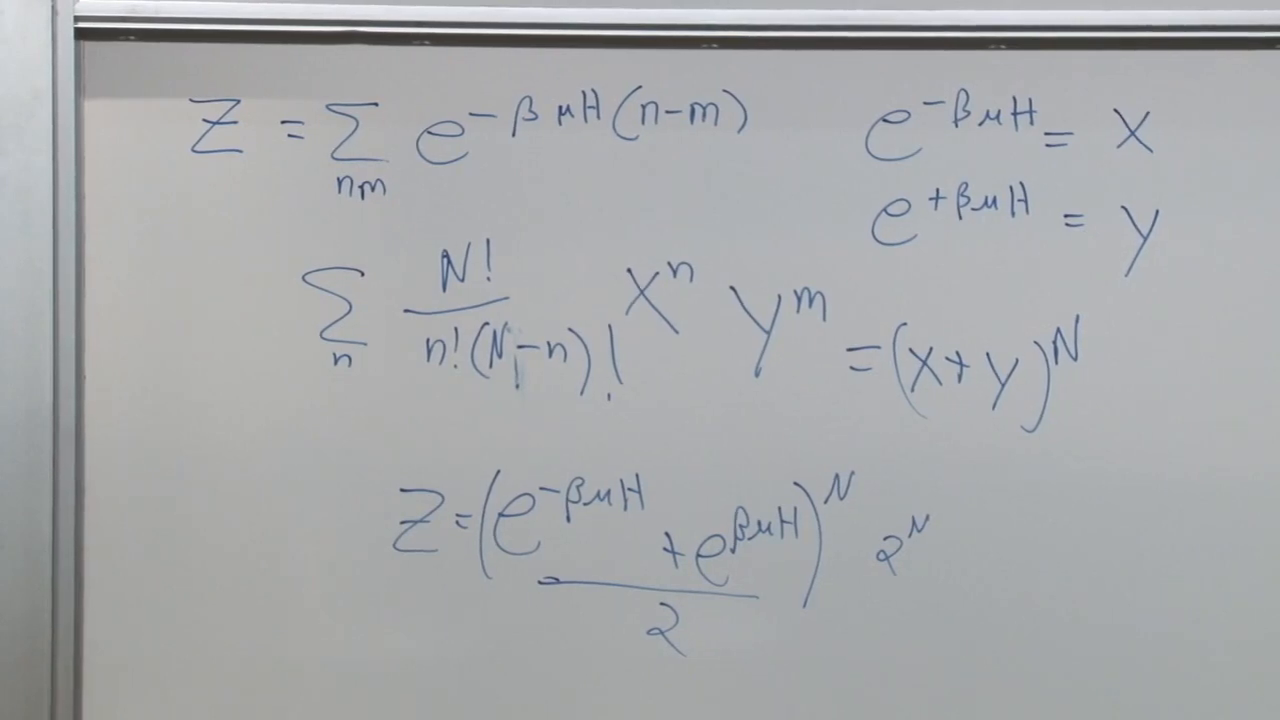
\includegraphics[width=0.90\textwidth]{lecture_08_figure_04.png}
\caption{分配関数の和、置換\(x\)および\(y\)、そして\(2\cosh(\beta\mu H)\)の冪への二項定理による簡約。}
\lectureframe{00:56:00}
\end{figure}

より短い導出もある。スピンは独立であるから、一つのスピンは
\begin{equation}
 z_1=e^{-\beta\mu H}+e^{+\beta\mu H}
    =2\cosh(\beta\mu H),
 \label{eq:sm8-one-spin-z}
\end{equation}
および\(Z_N=z_1^N\)を持つ。それでも組合せによる導出は、多重度がエネルギーとどのように競合するかを明示的に示すので、保持する価値がある。

\section{配置の磁化とアンサンブルの磁化}

一つの配置に対して、そのサイトあたりの無次元スピン過剰を次で定義する：
\begin{equation}
 M_{\rm conf}=\frac{n-m}{N}.
 \label{eq:sm8-config-magnetization}
\end{equation}
これはすべてのスピンが上向きのとき\(+1\)から、すべてのスピンが下向きのとき\(-1\)までの範囲をとる。ここで用いる熱力学的磁化はそのボルツマン平均であり、
\begin{equation}
 M=\left\langle M_{\rm conf}\right\rangle
  =\left\langle\frac{n-m}{N}\right\rangle.
 \label{eq:sm8-average-magnetization}
\end{equation}
因子\(\mu H\)はこの定義に属さない。計算中に一時的にそこに書かれ、その後除かれた。\(\mu H\)はスピン過剰をエネルギーに変換する。

配置ごとに、
\begin{equation}
 E=N\mu H M_{\rm conf}.
 \label{eq:sm8-energy-config-m}
\end{equation}
平均の線形性から直ちに
\begin{equation}
 \langle E\rangle=N\mu H M.
 \label{eq:sm8-energy-average-m}
\end{equation}

\begin{figure}[t]
\centering
\includegraphics[width=0.90\textwidth]{lecture_08_figure_05.png}
\caption{スピンの行、補正された平均磁化、そして黒板で強調されたエネルギー関係。}
\lectureframe{01:01:22}
\end{figure}

\begin{classroomqa}
\audiencequestion{磁化は特定の配置に割り当てられているのか、それとも平均磁化について議論しているのか。なぜ同じ関係が平均エネルギーに対しても成り立つのか。}
\lecturerresponse{両方の概念が現れるが、それらは区別されるべきである。\((n-m)/N\) は一つの配置における値であり、\(M\) はそのボルツマン平均である。\(E=N\mu H M_{\rm conf}\) は各配置で別々に成り立つので、両辺を同じ確率で平均すると \(\langle E\rangle=N\mu H M\) が得られる。固定された量 \(N\)、\(\mu\)、\(H\) は平均の外に出る。
\lecturetimestamp{00:59:54--01:03:40}}
\end{classroomqa}

\begin{classroomqa}
\audiencequestion{どのようにしてモデルは、上向きと下向きの間に偏りを与えることなく、すべてのスピンを北--南に揃えることができるのか。}
\lecturerresponse{東と西が存在しないことは二状態モデルに組み込まれている。それは許される自由度の制限である。現在の外部場モデル \emph{は}上向きと下向きの間に偏りを持つ。我々の符号の規約では、場は下向きスピンのエネルギーを下げる。したがってこのモデルには上--下対称性がない。以下で導入するゼロ場イジング模型がその対称性を回復する。
\lecturetimestamp{01:03:41--01:04:53}}
\end{classroomqa}

\subsection{分配関数からのエネルギー}

平均エネルギーは通常の恒等式から従う。
\begin{equation}
 \langle E\rangle
 =-\frac{\partial}{\partial\beta}\log Z_N.
 \label{eq:sm8-energy-identity}
\end{equation}
\eqref{eq:sm8-spin-z-closed} を用いると、
\begin{align}
 \log Z_N
 &=N\log 2+N\log\!\left[\cosh(\beta\mu H)\right],
 \notag\\
 \langle E\rangle
 &=-N\mu H\,
   \frac{\sinh(\beta\mu H)}{\cosh(\beta\mu H)}
 \notag\\
 &=-N\mu H\tanh(\beta\mu H).
 \label{eq:sm8-average-energy}
\end{align}
これを \eqref{eq:sm8-energy-average-m} と組み合わせると
\begin{equation}
 \boxed{M=-\tanh(\beta\mu H)}.
 \label{eq:sm8-magnetization-tanh}
\end{equation}

答えの形に物理が含まれている。思い出そう。
\begin{equation}
 \cosh x=\frac{e^x+e^{-x}}{2},
 \qquad
 \sinh x=\frac{e^x-e^{-x}}{2}.
 \label{eq:sm8-hyperbolic-definitions}
\end{equation}
原点付近では \(\tanh x=x+O(x^3)\) であり、大きな正の \(x\) に対しては \(1\) に近づく。\(\beta=1/T\) であるから、
\begin{equation}
 M\longrightarrow -1
 \quad (T\longrightarrow0),
 \qquad
 M\longrightarrow 0
 \quad (T\longrightarrow\infty).
 \label{eq:sm8-magnetization-limits}
\end{equation}
ゼロ温度ではすべてのスピンがより低いエネルギーの下向き状態を占める。無限温度ではすべての配置が等しい重みを持ち、場の偏りは洗い流される。\(H\) を反転させると \(M\) が反転する。

\begin{figure}[t]
\centering
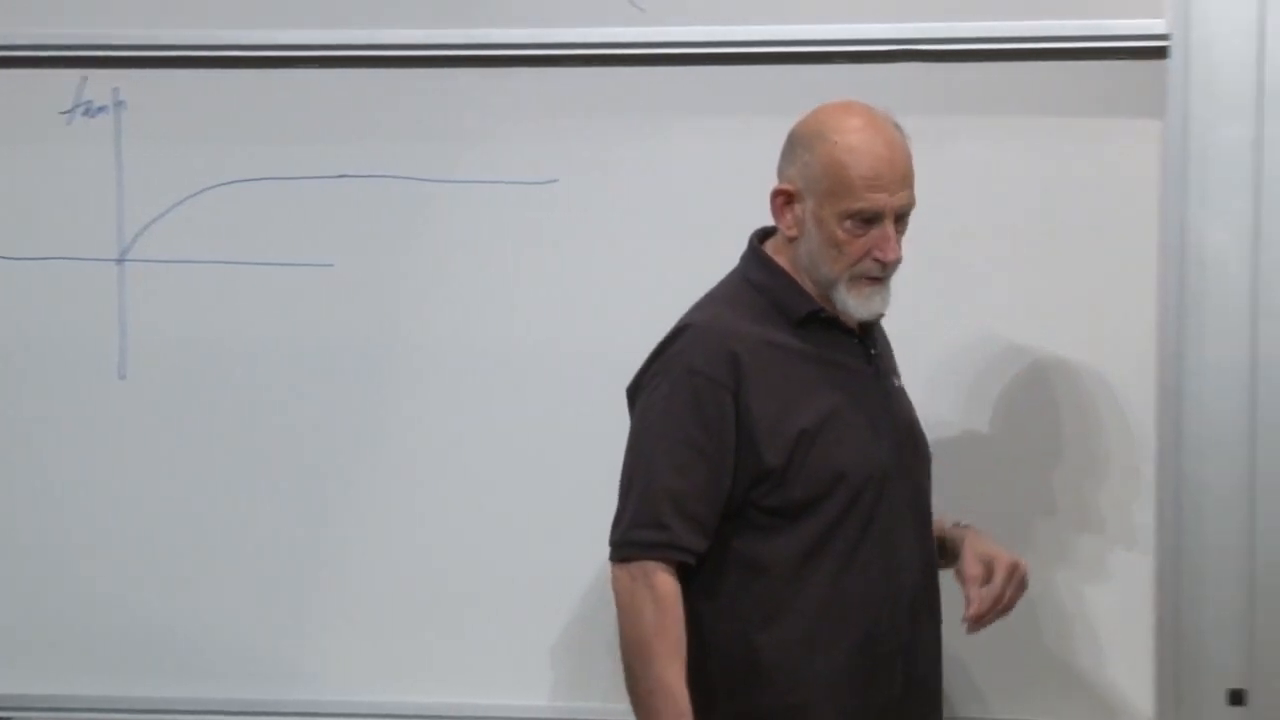
\includegraphics[width=0.90\textwidth]{lecture_08_figure_09.png}
\caption{双曲線正接曲線は大きな \(\beta\mu H\) で一定値に近づき、原点付近では線形である。講義の規約における物理的磁化は、プロットされた \(\tanh\) の負である。}
\lectureframe{01:13:14}
\end{figure}

\begin{classroomqa}
\audiencequestion{磁化は連続的に変化する。先に言及された相転移温度はどこにあるのか。}
\lecturerresponse{このモデルには存在しない。非零の外部場中の独立スピンは単純すぎ、\(\log Z_N=N\log[2\cosh(\beta\mu H)]\) はすべての有限の正の温度で滑らかである。相転移には、今から取り組む相互作用する対称な問題が必要であり、二次元ゼロ場イジング模型が有限温度転移を持つこの族の最初の例である。
\lecturetimestamp{01:14:47--01:15:11}}
\end{classroomqa}

\section{イジング模型：隣接ペアのエネルギー}

外部場は統計が始まる前に方向を選んだ。その場を取り除き、隣接スピンが互いの有効場を提供するようにしよう。あるサイトの両隣が上を向いていれば、それらは上を好む。両方が下を向いていれば、下を好む。一方がそれぞれ逆を向いていれば、最も単純な描像ではそれらの効果は打ち消し合う。エネルギーは今や孤立したサイトではなくペアに結びついている。

二つの隣接スピンに対して、\(J>0\) を選び、
\begin{equation}
 E_{12}=-J\sigma_1\sigma_2.
 \label{eq:sm8-pair-energy}
\end{equation}
と書く。揃ったスピンは \(\sigma_1\sigma_2=+1\) を持ち、エネルギーは \(-J\) である。逆向きのスピンは積 \(-1\) を持ち、エネルギーは \(+J\) である。したがってマイナス符号こそが相互作用を強磁性的にするものである。

\begin{figure}[t]
\centering
\includegraphics[width=0.90\textwidth]{lecture_08_figure_06.png}
\caption{局所強磁性相互作用
\(E_{12}=-J\sigma_1\sigma_2\)。}
\lectureframe{01:19:59}
\end{figure}

開いた一次元鎖ではハミルトニアンは
\begin{equation}
 {\cal H}=-J\sum_{i=1}^{N-1}\sigma_i\sigma_{i+1}.
 \label{eq:sm8-ising-chain-open}
\end{equation}
である。周期境界条件では \(\sigma_{N+1}=\sigma_1\) と置き、\(N\) まで和を取る。どちらの規約でも各隣接ペアを一度ずつ数える。それらの境界の違いは長い鎖では無視できるようになる。

\begin{figure}[t]
\centering
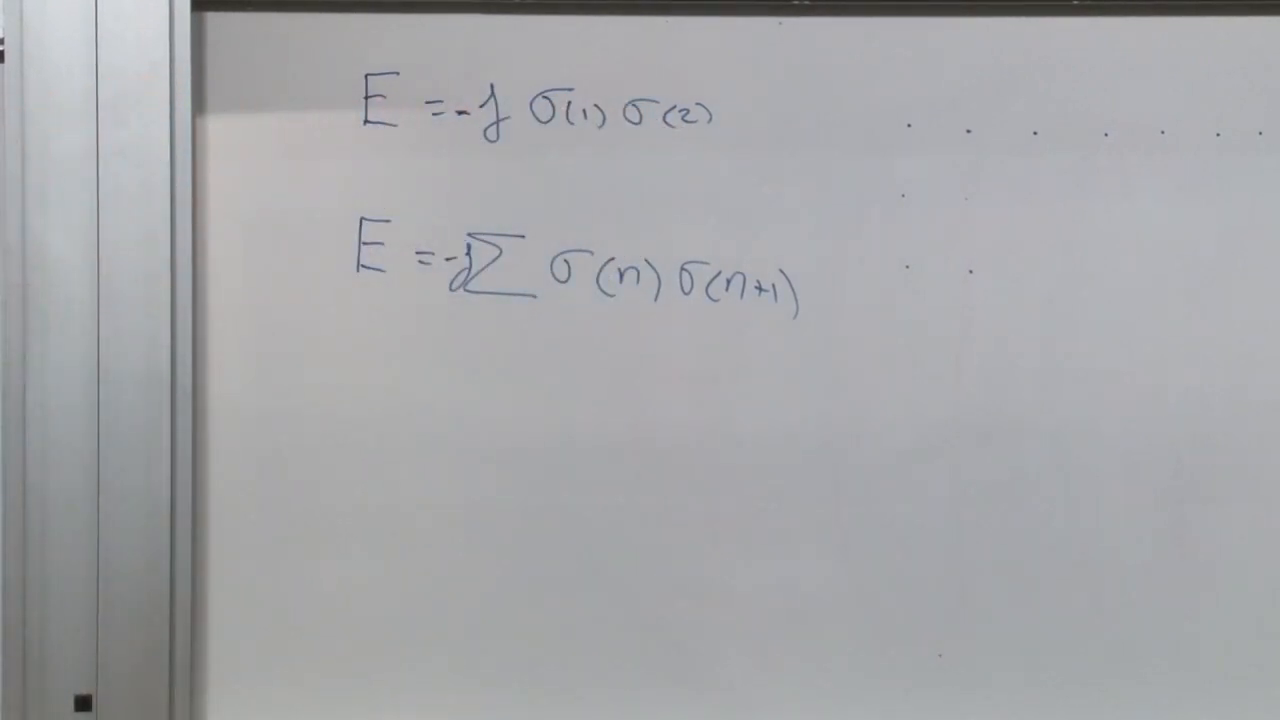
\includegraphics[width=0.90\textwidth]{lecture_08_figure_10.png}
\caption{局所ペアエネルギーを最近接鎖ハミルトニアンに拡張したもの。}
\lectureframe{01:20:46}
\end{figure}

無限温度ではすべてのスピン列が等確率である。平均して結合の半分は揃っており、半分は逆向きであるから、
\begin{equation}
 \left\langle\sigma_i\sigma_{i+1}\right\rangle_{T=\infty}=0,
 \qquad
 \left\langle{\cal H}\right\rangle_{T=\infty}=0.
 \label{eq:sm8-infinite-t-bond}
\end{equation}
ここでのゼロエネルギーは低エネルギー状態ではない。すべて揃った基底状態は結合あたりエネルギー \(-J\) を持つので、無限温度のアンサンブルはそれより示量的なエネルギーだけ上にある。

\begin{classroomqa}
\audiencequestion{個々の積 \(\sigma_i\sigma_{i+1}\) が \(+1\) か \(-1\) のいずれかであるのに、なぜ平均積がゼロになりうるのか。}
\lecturerresponse{平均は単一配置で取られる値の一つである必要はない。無限温度では揃った結合と逆向きの結合が等しい頻度で起こるので、それらの \(+1\) と \(-1\) の寄与は打ち消し合う。磁化で重要だったのと同じ平均の区別がここでも重要である。
\lecturetimestamp{01:21:39--01:22:37}}
\end{classroomqa}

\subsection{二つの基底状態と一つの大域的対称性}

絶対零度では、すべての結合が揃おうとする。したがって二つの基底状態が存在する。
\begin{equation}
 (+,+,+,\ldots,+)
 \qquad\hbox{and}\qquad
 (-,-,-,\ldots,-).
 \label{eq:sm8-two-ground-states}
\end{equation}
これらはまったく同じエネルギーをもつ。ハミルトニアンはこの縮退を明瞭にする。すなわち、すべてのスピンを反転させると、
\begin{equation}
 \sigma_i\longmapsto-\sigma_i
 \qquad\hbox{for all }i,
 \label{eq:sm8-global-flip}
\end{equation}
すべての結合の積は不変である。
\begin{equation}
 (-\sigma_i)(-\sigma_{i+1})
 =\sigma_i\sigma_{i+1}.
 \label{eq:sm8-global-flip-invariance}
\end{equation}
一つのスピンを反転させることは対称性ではない。なぜなら、隣接する結合の積の符号を反転させるからである。すべてのスピンを反転させることは対称性である。これが零磁場イジング模型の大域的\(\mathbb Z_2\)対称性である。

\begin{figure}[t]
\centering
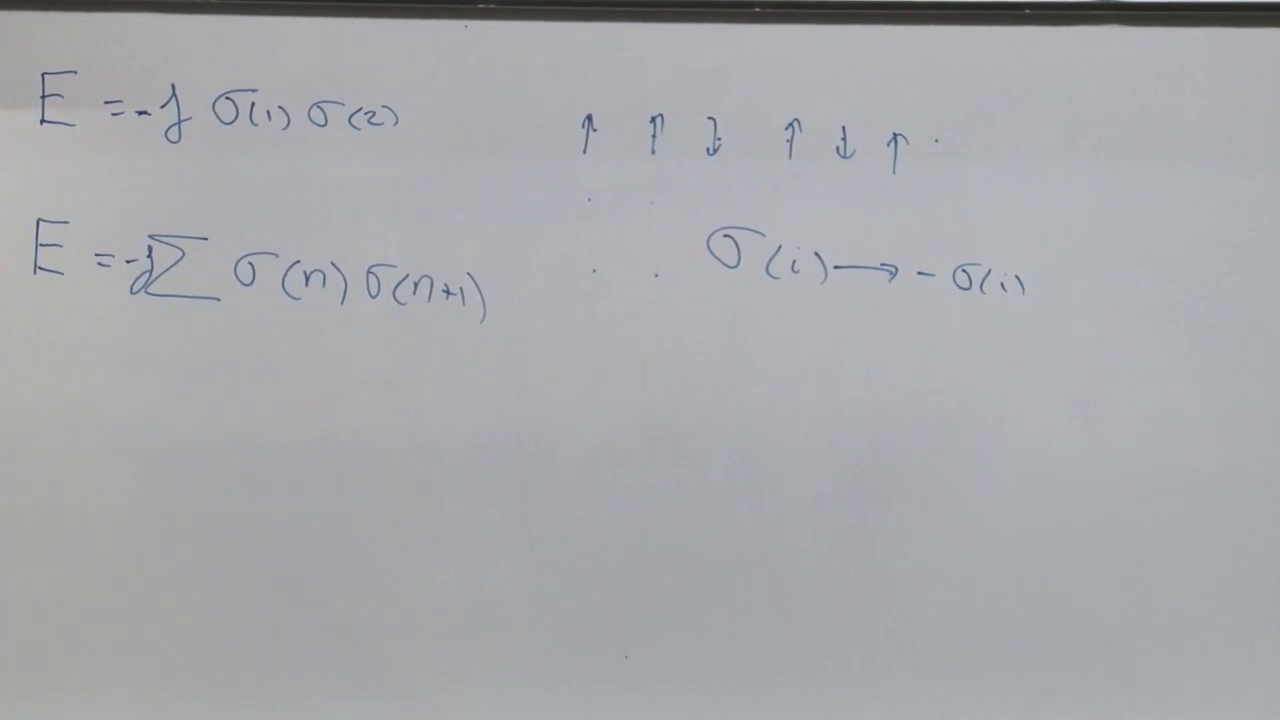
\includegraphics[width=0.90\textwidth]{lecture_08_figure_11.png}
\caption{大域的変換\(\sigma_i\mapsto-\sigma_i\)の隣に置かれた鎖のハミルトニアン。この変換はすべての対の積を不変に保つ。}
\lectureframe{01:26:31}
\end{figure}

厳密に絶対零度において、一つのスピンに微小な磁場を加える。それは二つの基底状態の間の引き分けを破り、強磁性的結合がその選択を鎖全体に伝播させる。状態が選択された後に磁場を取り除くと、大きな系はその配向を非常に長い時間保持しうる。これが自発的対称性の破れへの直観的な入り口である。

ここには一つの本質的な統計的但し書きがある。厳密に零磁場にある有限系では、正準集団は二つの基底状態に等しい重みを与え、したがって平均磁化は零である。対称性の破れた相は、選択磁場を取り除く前に熱力学的極限をとることによって定義される。
\begin{equation}
 M_*=\lim_{H\to0^+}\lim_{N\to\infty}M_N(H).
 \label{eq:sm8-order-of-limits}
\end{equation}
一次元最近接模型では、この極限は\(T=0\)においてのみ非零である。有限温度は無限鎖における長距離秩序を破壊する。二次元では、秩序相は非零の臨界温度以下で生き残る。

\subsection{歴史的訂正}

教室での説明は、この歴史をイジングを揶揄する冗談とともに語る。正確な年代順はもっと親切である。ヴィルヘルム・レンツがこの模型を提案し、彼の学生エルンスト・イジングが1924年の学位論文で一次元の場合を解いた。それは1925年に出版された。イジングは一次元では有限温度の強磁性転移が存在しないことを正しく見出したが、より高次元のより広い意義はまだ理解されていなかった。クラマースとワニエは二次元の双対性を発展させ、1941年に正方格子の臨界点を同定した。オンサーガーは1944年に有名な厳密な零磁場解を与えた。

次の計算は今や明瞭である。我々は\eqref{eq:sm8-ising-chain-open}の分配関数を求め、その相関が温度にどのように依存するかを決定しなければならない。その計算は、一次元鎖に有限温度の相転移が存在しない理由と、次元性がなぜ重要であるかを明示的に示すであろう。

\section{現在の位置づけ}

再帰の問題とスピンの問題は、同じ統計的教訓の二つの版である。気体では、エントロピーの不足がマクロ状態を指数的に稀にする。
\begin{equation}
 P(A)=e^{-\Delta S},
 \qquad
 \tau_{\rm rec}\sim\tau_{\rm mix}e^{\Delta S}.
 \label{eq:sm8-summary-recurrence}
\end{equation}
可逆な力学は回帰を許すが、巨大な相体積比が、通常の経験がなぜ緩和のみを見るのかを説明する。残る時間の矢の問題は、特別な宇宙論的初期条件にあり、微視的可逆性の失敗にあるのではない。

磁場中の独立なスピンに対して、
\begin{equation}
 Z_N=\left[2\cosh(\beta\mu H)\right]^N,
 \qquad
 M=-\tanh(\beta\mu H).
 \label{eq:sm8-summary-spins}
\end{equation}
その系は明示的にバイアスがかけられており、温度とともに滑らかに変化する。イジング相互作用
\begin{equation}
 {\cal H}=-J\sum_i\sigma_i\sigma_{i+1}
 \label{eq:sm8-summary-ising}
\end{equation}
は外部バイアスを取り除き、大域的アップ--ダウン対称性を回復し、真の秩序化の問題を提示する。すなわち、対称な多体系は非零温度で二つの秩序状態の一方を選ぶことができるか、という問題である。